\chapter{Proposed approach}
\label{chap:proposed_approach}
	\textit{This chapter displays the problems as well as the malicious request validator's input and output. Then we offer the design and architecture of the problem's solutions.}
\minitoc

\section{Cyber security problems}
\label{Cyber problems}
WAFs\index{WAF}, as previously indicated, are frequently used, however, they suffer from high false positive\index{False positive}. We aim to enhance the accuracy\index{Accuracy} of WAFs, using the help of machine learning\index{Machine learning (ML)} rather than rule-based\index{Rule-based} approaches.  \\
Because WAFs only cover the Application Layer, the network requests are the model's input (mostly HTTP requests). Our methodology produces the same result as WAFs: whether the request is malicious or not.\\
With its nature, WAF is obligated to have fast processing speed in deciding whether an incoming request is reliable or not. For user experiences, we can't examine the request's veracity for minutes before granting or denying access. Our system's time constraint must be in milliseconds.\\
Any flaw in an organization's internal controls, system procedures, or information systems is known as a vulnerability in cyber security. Cybercriminals may target these vulnerabilities and exploit them through the points of vulnerability.
These hackers can enter the networks without authorization and seriously harm data privacy. As a result, it is crucial to constantly check for cybersecurity vulnerabilities because flaws in a network could lead to a complete compromise of an organization's systems.
Let's take a look at some common cybersecurity vulnerabilities\footnote{
    Intellipaat. \textit{What is Vulnerability in Cyber Security? Types and Definition}.
    Mar 2023.
    \url{https://intellipaat.com/blog/vulnerability-in-cyber-security/}
}:
\begin{itemize}
    \item \textbf{Zero-day vulnerabilities}
    Zero-day vulnerabilities are specific software flaws that the attackers are aware of but that a company or user hasn't yet discovered.
    Since the vulnerability has not yet been identified or reported by the system manufacturer, there are no known remedies or solutions in these situations. These are particularly risky because there is no protection against them before an attack occurs. To reduce the risk of zero-day attacks, it is crucial to exercise caution and constantly check systems for vulnerabilities.
    \item \textbf{Poor Encryption}
    If a network has weak or nonexistent encryption, it will be easier for attackers to intercept system communications and compromise them. Cybercriminals may obtain crucial information and introduce misleading information onto a server when there is weak or unencrypted data. This may result in regulatory body fines and adversely jeopardize an organization's efforts to comply with cyber security regulations.
    \item \textbf{System misconfigurations}
    System failures can be caused by network assets with inappropriate security settings or restrictions. Networks are frequently searched for system errors and vulnerable spots by cyber criminals. Network misconfigurations are increasing as a result of the quick digital revolution. Working with knowledgeable security professionals is crucial when implementing new technology.

\end{itemize}

\section{Ratiocination}
\label{ratio}
To summary, numerous strategies for identifying malicious URLs have been proposed. Most of these solutions utilize supervised-based machine learning\index{Machine learning (ML)} techniques for classification. This technique can detect irregularities between requests, but it cannot extract these abnormalities into human-readable form in order to reconstruct the WAF\index{WAF}. Relying solely on machine learning eventhough brought higher accuracy\index{Accuracy} like in \cite{s22093373}, WAFs need to be time-efficient. We can not compromise accuracy for speed, hence these methods don't work for WAFs.\\
We come to the approach is to categorize the incoming request and analyze its structure, with moderate reliability, then combining the result of these two process to achieve the high precision\index{Precision} yet does not expending an excessive amount of time.

We have some theoretical points to prove why we decide to design in this way: \\
\textbf{First point,} in his 1996 paper, The Lack of A Priori Distinctions Between Learning Algorithms, D. H. Wolpert introduced the No Free Lunch theorem for supervised machine learning and stated a quote at the beginning of his paper. The theorem states that given a noise-free dataset, “for any two machine learning algorithms A and B, the average performance of A and B will be the same across all possible problem instances drawn from a uniform probability distribution.” This means  “an algorithm may perform very well for one problem, but that gives us no reason to believe it will do just as well on a different problem where the same assumptions may not work.” \\
\textbf{Second point,} moreover, simpler models like logistic regression\index{Logistic regression} have more bias and tend to underfit, while more complex models like neural networks have more variance and tend to overfit. \\
\textbf{Strengths and Weaknesses of Logistic Regression:} 
Let's take a look at some advantages provided by Logistic Regression. Firstly, it's easy to deploy, and it calculates accurately and fasts with big data. Secondly, it can handle both continuous and discrete data. Next, it's suitable for binary or multiclass classification problems. Finally, it allows us to determine the importance of input features. Besides the strengths, this model also has some weaknesses.
First, this model cannot deal with data that is non-linear or has complex linear relationships. Second, it is sensitive to noise and outliers in data. Next, it can only be applied to classification problems, not to unsupervised learning algorithms. Lastly, it is prone to overfitting when the number of features is larger than the number of training samples.

\textbf{Strengths and Weaknesses of CNN:} 
CNN\index{CNN} model combined with word2vec\index{word2vec} is a widely used method in Machine Learning to perform natural languages processing tasks such as text classification or machine translation. Below is a detailed analysis of the strengths and weaknesses of the CNN model combined with word2vec.
Let's look at some of the CNN model's benefits. First, it can handle ordered data, including long data strings. Second, it can remember past information and apply it to future decisions. Next, it helps machine learning models understand the meaning of words and sentences in natural language. Another advantage, this model is capable of learning common features from texts, resulting in better prediction results with never-before-seen new text. Finally, CNN is faster by design compared to RNN - the more fitting model to categorize text. This machine learning model also has some weaknesses. The first one is that the CNN model requires a lot of computational resources to train due to many parameters. The following disadvantage is that sometimes it is not effective for problems with complex structured data such as images. Next, it is necessary to use appropriate dictionaries to represent words in vector space. Eventually, it is difficult for it to deal with words that are not in the user dictionary. 

\textbf{Last point,}
Ensemble learning\index{Ensemble learning} is an approach that combines diverse models to improve performance. The idea behind integrating different models is logical: each model has unique abilities, and when combined, they may excel in multiple tasks or subtasks. When these models are appropriately merged, they create a potent training algorithm capable of enhancing overall performance compared to using individual models alone.
Ensemble learning reduces variance and bias, improving predictions of the developed model. Technically speaking, it helps avoid overfitting.

This problem classifies the input data as yes/no. It needs accuracy\index{Accuracy} and the data set is not large, needs high accuracy. So we decided to combine logistic regression\index{Logistic regression} and CNN\index{CNN} model.

\emph{Comparisons between ensemble learning and other machine learning approaches} \\
To prove that ensemble learning is good enough for our project, we will make comparisons between ensemble learning and other machine learning\index{Machine learning (ML)} approaches.
First, let's discuss ensemble and rule-based\index{Rule-based} learning. About the method, ensemble learning is a method of combining different machine learning models to create a better predictive model, while rule-based learning is a method of determining specific security rules based on information about known web attacks. About performance, ensemble learning can improve the performance of a machine learning model because it aggregates predictions from many different models. Meanwhile, new or unknown attacks can easily bypass rule-based learning. One of the most importance aspects is accuracy,
ensemble learning can improve the accuracy of machine learning models by eliminating false predictions. However, the accuracy of the ensemble learning model also depends on the combination of submodels. Rule-based learning can achieve high accuracy if security rules are set up correctly.
About generalizability, ensemble learning can improve the generalizability of a machine learning model by using a variety of models and avoiding overfitting. Rule-based learning may not generalize well if the security rules are not universal enough or easily circumvented. In summary, ensemble learning can improve the performance, accuracy, and generalizability of machine learning models for WAFs\index{WAF}. Meanwhile, rule-based learning provides specific security rules and achieves high accuracy in some cases.

Another approach that comes into discuss is deep learning-based. Deep learning-based method has some advantages. First, deep learning uses complex models to analyze data, making it possible to learn and process data more accurately. Second, it is capable of handling and classifying thousands of attack types. Finally, it has the ability to automate the updating of security rules. Besides the strengths, it also has some limitations. The first limitation is that it requires large and varied training data to produce accurate results. Next, it requires powerful hardware to train and deploy the model. Lastly, it is difficult to explain how deep learning models work. 

Thus, deep learning and ensemble learning both have their own advantages and disadvantages. However, because the special nature of WAF is often to protect against new attacks, ensemble learning may be the better choice due to its ability to detect new attacks based on a combination of models.

\section{Designs}
\label{design}
There are many efforts spent on this topic, as mentioned in section (Related works).But there are two significant literatures about detecting malicious requests that inspired us: \\
1. Mohammed Alsaedi et al\cite{s22093373} proposed an approach to detect malicious URLs using ensemble learning\index{Ensemble learning}. They extracted features using N-Gram and then use TF-IDF\index{TF-IDF} to represent them. After that, the model applied Rain Forest Ensemble-Based for prediction and an artificial neural network (ANN) classifier was constructed for decision making. Results show that this approach significantly improved the detection performance, achieving 96.80\% compared with the best 90.4\% achieved by the URL-based features. The false-positive rate was significantly decreased to 3.1\% compared with 12\% performed by the URL-based model. This work is proven to be promising, but time is not the focus of this approach. \\
2. Khoi. Le et al\cite{Khoi} suggested an approach of extracting WAF\index{WAF} rules and trained a machine learning\index{Machine learning (ML)} with the decision model independent from the rules themselves. This makes the model more self-reliant and the overall result more neutral. The module has been tested, and though it is not completed yet, it shows potential. We aim to finalize this module but combine it with another machine learning model to specialize it for the goal of determining incoming requests independent of the WAF rule.

Our proposed approach is explained as follow:

It is already obvious that when attackers attempt to breach a system, they must try to execute or inject something executable onto the system. Malicious requests must therefore be script-based or written in computer languages. Most standard online applications and services, particularly API applications, appear to accept just plain text queries, i.e. requests in JSON or XML. 
In the event of a website service that accepts scripted input, certain malicious requests may have the same category or language as the normal request; for example, the attacker may alter the SQL database account using SQL queries ('normal' database server category). However, the content of the malicious request seems to have a similar pattern. Moreover, to gain access to executing queries, attackers must try various methods to penetrate the server (reconnaissance scan, code injection, or command injection on the back-end servers and database servers). Then we only need to detect one malicious request to block all the attack session. Of course, WAF cannot protect systems from high-level methods, for example, attackers gain access by acquiring admin accounts from social engineering.

Our goal is to classify request supplied as inputs in order to determine whether they are harmful or inoffensive. The sample of request data consists of different categories including:
\begin{itemize}
    \item \emph{Plain text}: request that contains data but does not trigger any machine execution, typically in the form of HTML, JSON, XML, and CSV, etc.
    \item \emph{Client-side script}: request in form of programming languages or scripts that can be executed on client's machine.
    \item \emph{Server-side script}: request in the form of programming languages (mostly back-end programming languages like PHP, JAVA, PYTHON, and so on) that can change the behavior of the application or web.
    \item \emph{Shell script}: request in the form of shell scripts that can run jobs on the server or change the server's or operating system's behavior.
    \item \emph{SQL script}: request that in form of SQL, can be used to query data from the database.
\end{itemize}

Then we introduce the first hypothesis: normal requests to a server have the same category. For example, a static web request may only contain plain text, API server requests are mostly in JSON format, incoming queries to a database are SQL or online compilers use programming language-format requests. A malicious request must be in different category with the normal requests, like a script request to a static web server or API server can be considered code injection or command injection, SQL requests to an API server may be SQLi\index{SQLi}, or script requests to a database is command injection or stored XSS\index{XSS} attacks. We can determine if a request is 'normal' to a server by comparing the types of incoming suspicious requests to the average categories of regular requests. If the resemblance is low, we might presume that the origin of the inbound request is unusual. For instance, if a typical request to a secured server is in JSON format (plain text), but a suspicious request is in JavaScript (client-side script), we can deduce that the incoming request is malicious. If a suspicious request is in XML format (plain text), we may assume that the user made a mistake and the alarm was false.



The second hypothesis can be presented as all regular requests will have a similar pattern, the same goes for malicious requests. For example, a request with a URL ending in.exe or.php is frequently malicious, and a request with work like "SELECT", "DROP", or "TABLE" is unquestionably a SQLi. We can implement Logistic Regression\index{Logistic regression} to identify if an incoming request is normal or abnormal by analyzing its content.

From the hypothesises, we can create a CNN\index{CNN} model to detect the type of request. Then we compare the incoming requests with the "normal" corresponding category and decide whether the requests is malicious or not using Logistic regression.


\section{Architecture}
\label{architecture design}

Our architecture is described in the below figure (Figure 13). Suggest a reasonable decision model for the combined 
\begin{figure}[!h]
   
     \centering
     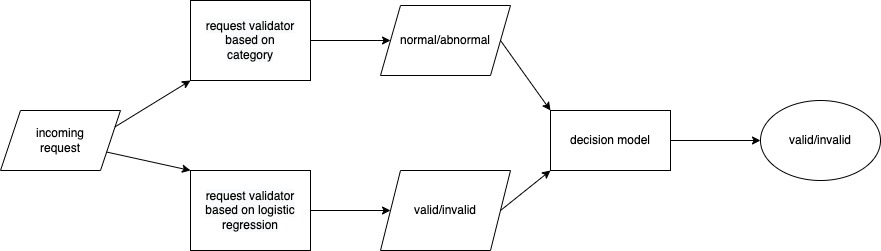
\includegraphics[width=\linewidth, height=10cm,keepaspectratio]{figures/architecture.jpg}
   \caption{Malicious request validator architecture}
\end{figure}
result: When two prediction is the same, the result is straight forward. When the logistic regression model decided that the request is malicious, but the CNN model predicted the request is nornal, the CNN is favored. Otherwise, the Regression model classified the request as valid but the CNN predicted as abnormal, we'll favor the Regression. The desicion model can be expressed in a decision table: \\

\begin{table}[h]
\begin{center}
\begin{tabular}{||c c c ||} 
 \hline
 Regression & CNN & Result  \\ [0.5ex] 
 \hline\hline
 Valid & Normal & Valid \\ 
 
 Valid & Abnormal & Valid  \\

 Invalid & Normal & Valid  \\
 
 Invalid & Abnormal & Invalid  \\ [1ex] 
\hline
\end{tabular}
\end{center}
\caption{\label{demo-table}Table 4.1}
\end{table}

The CNN validator will run for a set period of time (usually one or two weeks) to collect the familiar category of incoming requests and assign a threshold (which can be the mean or maximum (if we are optimistic) distance between each request vector in the observing stage and the sum vector). The same will also happened with the Regression model. After that training phase, the module will run on 'active phase', parallel with the WAF. 

\begin{figure}[!h]
     \centering
     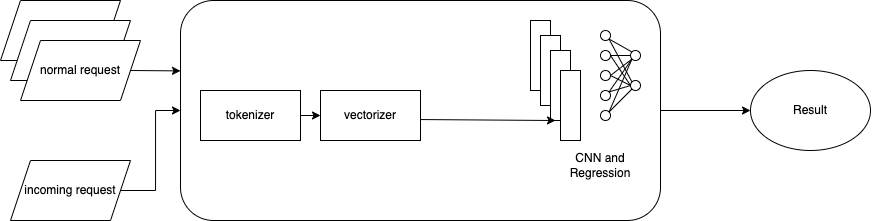
\includegraphics[width=\linewidth, height=10cm,keepaspectratio]{figures/architecture 2.drawio.png}
   \caption{Decision model for the combination of CNN and the Regression model}
\end{figure}

The request is routed through the module, which predicts the category. The category of suspicious request is then compared with the common category. Then the Regression model will determined whether the request is good or bad, combining with the normal or abnormal status to decide the result. 
